\documentclass[12pt]{exam}
\usepackage[utf8]{inputenc}
\usepackage[margin=1in]{geometry}
\usepackage{amsmath,amssymb}
\usepackage{multicol}
\usepackage{url}
\usepackage{graphicx}


\PassOptionsToPackage{hyphens}{url}\usepackage{hyperref}
\newcommand{\class}{Robot Intelligence}
\newcommand{\term}{Fall 2022}
\newcommand{\examnum}{Midterm Exam}
\newcommand{\examdate}{8/31/2022}
\newcommand{\timelimit}{10/28/2022}

\pagestyle{head}
\firstpageheader{}{}{}
\runningheader{\class}{\examnum\ - Page \thepage\ of \numpages}{\examdate}
\runningheadrule


\begin{document}

\noindent
\begin{tabular*}{\textwidth}{l @{\extracolsep{\fill}} r @{\extracolsep{6pt}} l}
\textbf{\class} & \textbf{Name:} & \makebox[2in]{\hrulefill}\\
\textbf{\term} &&\\
\textbf{\examnum} &&\\
\textbf{\examdate} &&\\
\textbf{Take Home Exam - Due Before Class on Canvas \timelimit} 
\end{tabular*}\\
\rule[2ex]{\textwidth}{2pt}

This exam contains \numpages\ pages (including this cover page) and \numquestions\ questions.\\
The total number of points is \numpoints. Graduate students must answer some additional questions. Undergraduates answering graduate questions will be given additional points and a feeling of satisfaction from attempting difficult things (probably). 

Any programming/code artifacts associated with this exam should be submitted along with the final PDF to canvas. Please put your entire submission in a single .zip file. 

This exam will cover topics in motion, planning, sensor processing, and ethics.


\begin{center}
    Grade Table (Quick view to see the breakdown)\\
    \addpoints
    \gradetable[v][questions]
\end{center}

\noindent
\rule[2ex]{\textwidth}{2pt}

\begin{questions}

\newpage

\addpoints
\question[20]
    Moving in a car 

   I would like you to use a skid steer model of a robot that is $75cm$ long and $55cm$ wide and run a few simple experiments with it. Please upload your resulting figures and python (or other) code: 
    
\noaddpoints
\begin{parts}
    \part[5] 
        Make a list of commands (at t=0.1) that will allow this robot to traverse the entirety of a $5m$ diameter circle. The robot starts off in the center of the circle (0,0) and you cannot leave the circles border. Plot the resulting path (x, y) and trajectory (x, y, and angular velocities). Assume constant velocity of $8 m/s$
    \part[5]
        Do the same as the above for a traditional car (Ackermann steering). 
    \part[10]
        If the car is traveling for $10s$, what is my position error using the discretized equations of motion if I define my time steps at $\Delta t = 1, 0.1, 0.01$ ? Plot the errors and computing time for each type of vehicle in these cases.
    
    \part[10] 
        \textbf{Graduate Student Question} Compute part c again where road frictions are much lower (due to rain or ice). Slip causes your tires to respond very differently. Assume that your theta is $\theta_{actual} = \theta (1 - 0.08)$ and velocity is $v_{actual} = v (1 - 0.04)$.
\end{parts}
\newpage


\addpoints
\question[20]
    Inverse Kinematics, numerical approaches
    
    The following SCARA-type manipulator has physical characteristics as follows: 
    $l_1 = 60cm$, $l_2 = 40cm$, and an arbitrary height (ie: assume that $(0,0)$ is at the first motor). 
    
\noaddpoints
\begin{parts}
    \part[5] 
        \begin{figure}
            \centering
            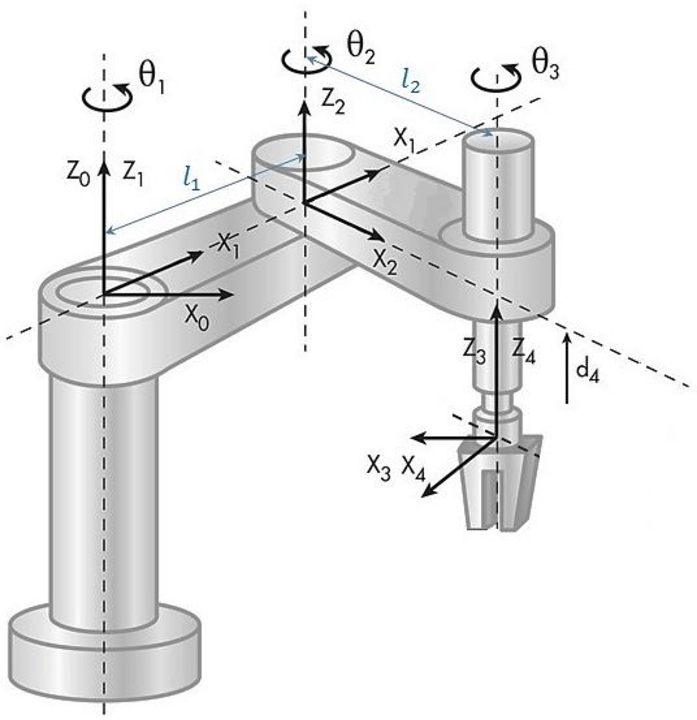
\includegraphics[width=0.5\textwidth]{SCARA-robot-of-4-gdl-Source-Our-elaboration.png}
            \caption{SCARA type manipulator. }
        \end{figure}
        
        What is the workspace volume for this robot?. (Draw a picture of it as well)
    
    \part[5] 
        Write the DH parameters 
    
    \part[10] 
        Compute the forward kinematics to find the position of the end effector if $\theta_1 = 30 deg$, $\theta_2 = 45 deg$, $\theta_3 = 90 deg$, and $d = 14 cm$
\end{parts}
\newpage


\addpoints
\question[20]
    Inverse Kinematics with numerical approaches (Use the manipulator on the following page). Note that $d_6$ refers to the length of the arm on the top and $d_1$ is the length of the system from the base to the first motor.)
    
    
\noaddpoints
\begin{parts}

    \part[10] 
        Compute the joint angles and extension distances that will get this robot to pick up an object at x=1.2, y=0.8, z=0.5 if the robot started at if the robot started with the end effector at $\theta_1= -90deg$, $d_2 = 0.5m$, $d_3 = 1.0m$, $\theta_4=-90deg$, $\theta_5 = 90deg$, $\theta_6 = 40deg$, $d_6 = 0.2m$.
        \begin{figure}
        \centering
        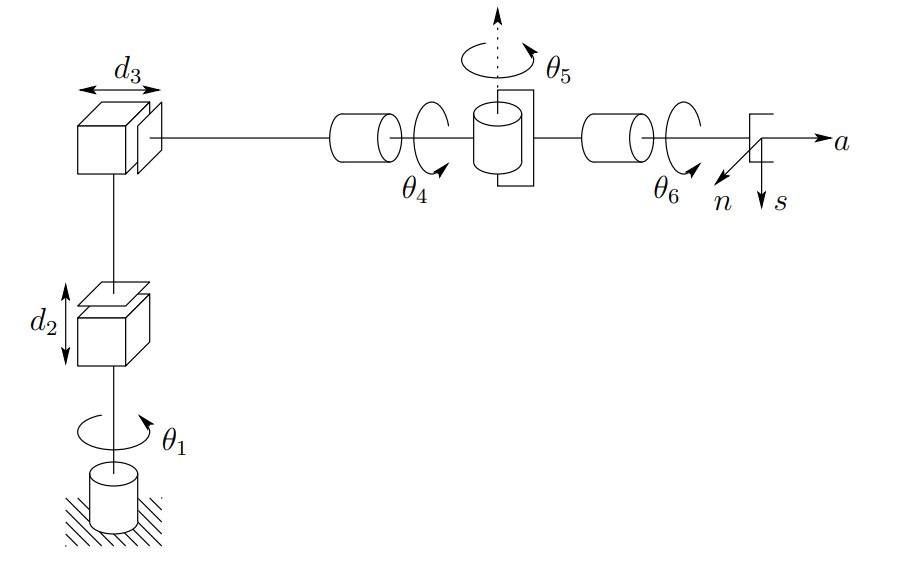
\includegraphics[width=0.5\textwidth]{6dof_arm.jpg}
        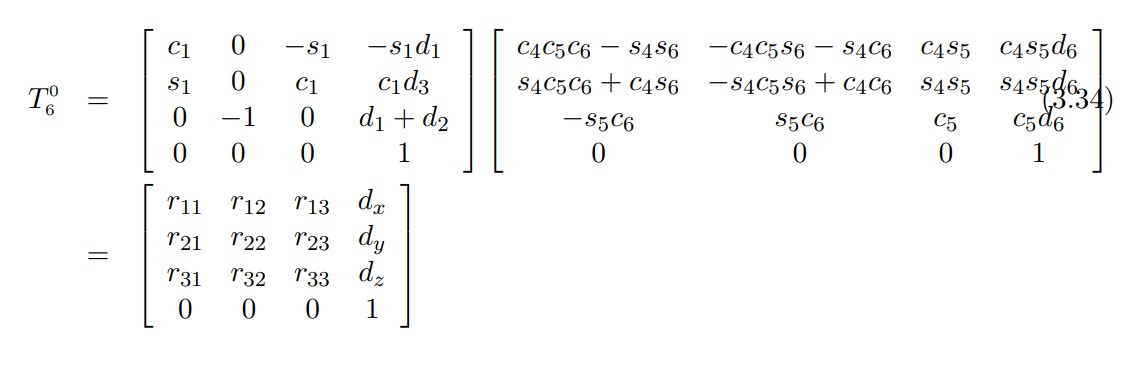
\includegraphics[]{6dof_arm_TMatrix.jpg}
        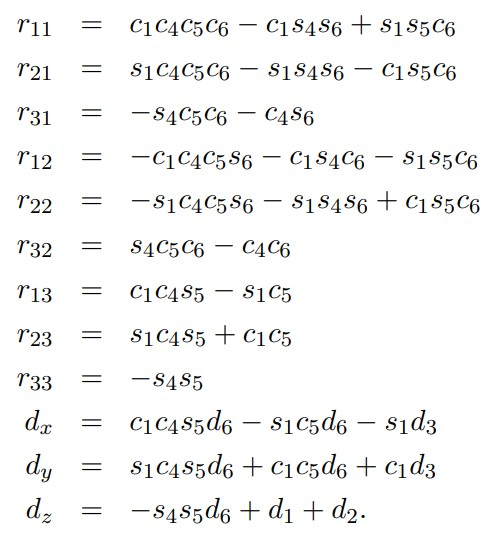
\includegraphics[]{6dof_arm_TMatrix_Eqs.jpg}
        \caption{Cylindrical/Prismatic manipulator. Use for problem 6.}
        \end{figure}
    
    \part[10] 
        What would be the joint angles and extension distances to get to the same goal coordinates if the robot started with the end effector at $\theta_1= -90deg$, $d_2 = 0.5m$, $d_3 = 1.0m$, $\theta_4=-90deg$, $\theta_5 = 90deg$, $\theta_6 = 40deg$, $d_6 = 0.2m$ and we wished to minimize the total distance traveled for each actuating part?
    
    \part[10]
        \textbf{Graduate Question:} Using the same system, start configuration, and goal coordinates, compute the energy-efficient joint angles and extension distances. For your energy model, assume that actuating $\theta_1$ costs 3x the energy of $\theta_{4,5,6}$, and $d_{2,3}$ costs 2x the energy.
    

\end{parts}
\newpage


\addpoints
\question[20]
    Balancing a Pole 
    
    A cart and pole suddenly appears before you and you feel compelled to answer burning questions you have always held about these systems. 

\noaddpoints
\begin{parts}
    \part[5] 
        \begin{figure}
            \centering
            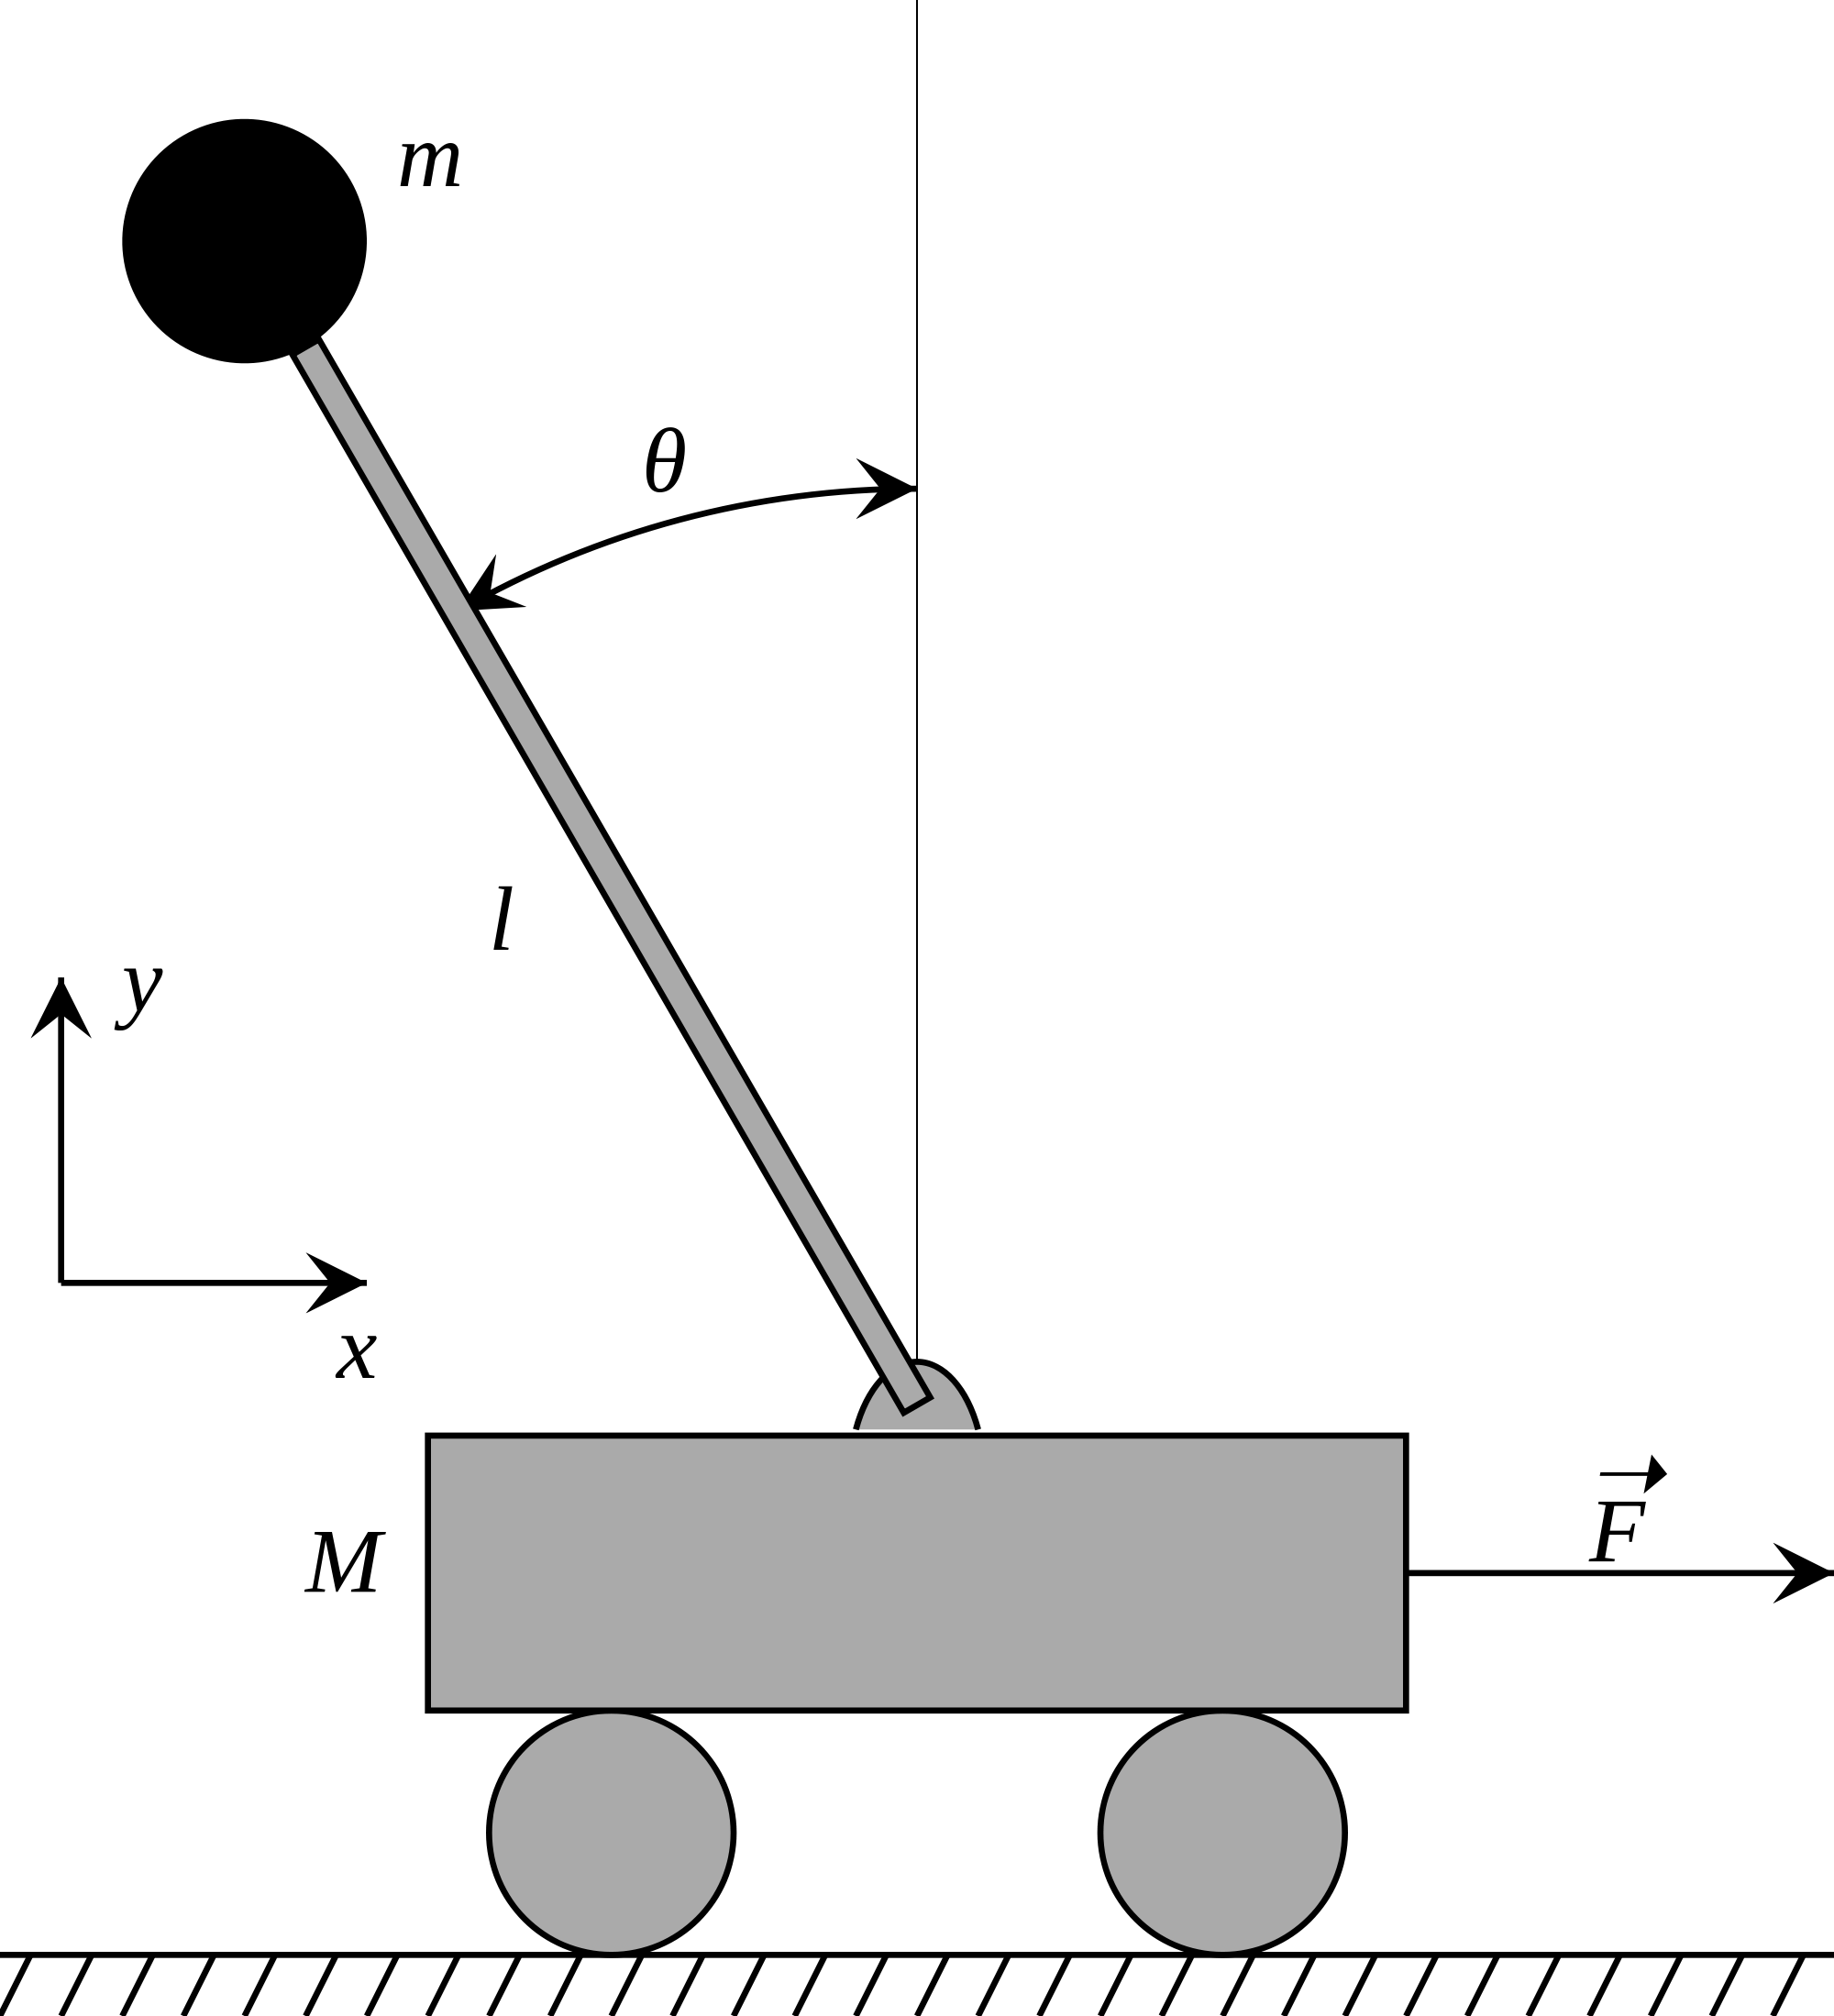
\includegraphics[width=0.5\textwidth]{cart-pole.png}
            \caption{Assume that the mass $m = 0.2kg$, $l = 1.0$, $M = 4.0kg$}
            \label{fig:cartpole}
        \end{figure}
        Describe the equations of motion that governs this system
        
    \part[10] 
        Generate code for a controller that would be able to keep the pole balanced in the air. 
        
    \part[5] 
        What is the maximum angle that my pole can fall to before it cannot recover if max Force $F = 6N $?
\end{parts}
\newpage

\addpoints
\question[20]

    Control and Reinforcement Learning
\noaddpoints
\begin{parts}
    \part[5] 
        Explain three merits and three demerits of using reinforcement learning for mechatronic systems.
    \part[5] 
        Draw a diagram for reinforcement learning and controls and contrast the two
    \part[10] 
         Use OpenAI Gym to create a trained reinforcement learning model for the cart and pole problem (CartPole-v1). 
    
        \url{https://www.gymlibrary.ml/environments/classic_control/cart_pole/}\\
    
        This tutorial will help you get started with using the OpenAI gym python library. \url{https://blog.paperspace.com/getting-started-with-openai-gym/}\\
    
    \part[10] 
    \textbf{Graduate Question:} Implement this example of a 2D running robot (cheetah) and adapt the code to penalize hip motor movements faster than $\pi \frac{rad}{s}$.  
        \url{https://github.com/openai/gym/blob/master/gym/envs/mujoco/half_cheetah.py} 
        A Virtual Machine that was made with VMWare is available on Canvas for you to use for this question if you have trouble installing Mujoco.

\end{parts}
\newpage



\addpoints
\question[20]
    Human Emotions

\noaddpoints
\begin{parts}

    \part[10] 
        Using the FER library in python, example in the following link:  \url{https://towardsdatascience.com/the-ultimate-guide-to-emotion-recognition-from-facial-expressions-using-python-64e58d4324ff}
        build a system that classifies human emotions and validate on video 1 and 2 from this repository: \url{https://github.com/rjrahul24/ai-with-python-series/tree/main/07.%20Emotion%20Recognition%20using%20Live%20Video}
        Generate plots of predicted emotions over time for both videos.

    \part[5]
        Do the same as the above with a video feed from your webcam. Set your software up to allow video feed or a pre-recorded video. (In essence, make faces at yourself and make sure that your service works). Submit a short faces-recording along with the script that can read live webcam streams. 
    
    \part[5] 
        What are the logical applications of this tool for an autonomous robot? What are the ethical and legal consequences of fielding a system that makes decisions based on this tool?

    \part[10]
        \textbf{Graduate Question:} Set up a service that allows 2 or more faces to be processed at once.
    

\end{parts}
\newpage

\addpoints
\question[20]
    Motion Planning

\noaddpoints
\begin{parts}

    \part[20] 
        Implement an A* based planner and compare it's results with the Djikstra, A-Star, RRT-Star, Bi-Directional A-Star, and the Breadth First Search Planners from this github. \url{https://github.com/AtsushiSakai/PythonRobotics/tree/master/PathPlanning}. 
        Create a table comparing the average cost of the path found over 10 iterations along with the time to convergence. 
    
        After you have implemented your planner and compared it answer the below questions. 
        \begin{itemize}
            \item Which planner provided a path with the lowest cost on average?
            \item Which one found a path the fastest on average? 
            \item After comparing your planner to these five other ones is there anything you would change in your planner to help it converge faster or find a path with a better cost?
            \item Which planner appears to be the best overall? Which planner would you use for a robot in a complex environment? 
        \end{itemize}
    
        % Could we just make the designing and building a planner the most important part of this? 
        % \part[10] 
            % Implement a skid-steer (4 wheel) vehicle model for a robot 33 inches wide, by 40 inches long for the planner that you chose.
    
    \part[10]
        \textbf{Graduate Question:} Take the RRT planner from \url{https://github.com/AtsushiSakai/PythonRobotics/tree/master/PathPlanning} and update it to be an RRT-Star algorithm.


\end{parts}
\newpage

\addpoints
\question[20]
    Object Detection (Please put the classified images as part of your submission)

\noaddpoints
\begin{parts}
    % Carter will solve this problem Yay! Agriculture might be great
    \part[5] 
        Classify the first 10 pictures in \url{https://github.com/ravirajsinh45/Crop_and_weed_detection} using any image classification algorithm.
    
    \part[5] 
        Implement Yolo and do the same, what are the differences. 
    
    \part[10] 
        Using transfer learning, pick an image classification algorithm and retrain it to learn to detect a new object of interest.

    \part[10]
        \textbf{Graduate Question:} Implement Detectron (\url{https://github.com/facebookresearch/Detectron}) and  test the image segmentation of the objects you are interested in. Give metrics on relative segmentation/classification quality comparing: Mask R-CNN, faster R-CNN, and RetinaNet.


\end{parts}


\newpage
\addpoints
\question[20]
    Full Circle - Car planning in a complex environment

\noaddpoints
\begin{parts}

    \part[5]
        A pedestrian suddenly begins to walk in front of the moving vehicle ($11 m/s$).  The pedestrian is 20 meters in front of the car. What commands will the car need to receive to stop before it hits the pedestrian? Plot the velocity, position, and commanded inputs. 
    \part[5] 
        Assume that your vehicle can only decelerate at $4.2 m/s^2$ (max). If there is an open lane to your left or right, generate a new stopping trajectory. Plot the velocity, position, and commanded inputs. 
    \part[5] 
        A New vehicle pulls out into the road 15 meters ahead of you and speeds up to $11 m/s$. Design a trajectory to pass on the left if your vehicle is moving at $13 m/s$. Plot the velocity, position, and commanded inputs. 
    \part[5]
        As you are passing the vehicle (where you begin to overlap), it speeds up to $13 m/s$. Compute a new passing trajectory if you are willing to accelerate to $14 m/s$, how much time will you be in a "Passing" maneuver? Plot the velocity, position, and commanded inputs. 

    % \part[10] \textbf{Graduate Question:}
    %     Traffic aware navigation - Your vehicle is stopped at an intersection making a left turn (yay). You are able to accelerate at 12 mph/s
    
    % \part[10]
    %     Using the autonomous driving dataset \url{https://www.nuscenes.org/nuimages#data-collection} combine sensors to build a spatial map of objects. Using Yolo and Python, build a visualization of all identified objects and their relative positions. 
        
    % \part[10]
    %     Integrate the CAN information using the nuscenes devkit \url{https://github.com/nutonomy/nuscenes-devkit}. 
    %     \begin{itemize}
            
        %     \part[10] \textbf{Graduate Question:} (Choose one) 
        %     Power aware navigation - Generate a power model of the vehicle to predict the power cost of maneuvers (hint, should be highly correlated with acceleration), and generate a route that optimizes the energy. 
            
        % \end{itemize}
        
\end{parts}
\newpage

\addpoints
\question[20]
    Ethics of Robotics - Open Ended Questions

\noaddpoints
\begin{parts}
    
    \part[5] 
        Many people (particularly those in the robotics industry) believe that robotics is purely within the purview of technical development and should not have any ethical considerations. What do you feel can be a merit or demerit to this way of thinking?
    
    \part[5] 
        Isaac Asimov listed 3 laws of robotics, comment on the algorithmic complexity of implementing these into working intelligence. Define a scenario and write Psuedo code to implement these rules. 
    
    \part[5] 
        In the event of an autonomous system causing harm or damages, who is responsible? Read and comment on the following two documents: \url{https://www.callahan-law.com/articles-and-expert-advice/when-an-autonomous-vehicle-hits-a-pedestrian-who-is-responsible/} and \url{https://en.wikipedia.org/wiki/Self-driving_car_liability}
    
    \part[5] 
        What laws may be helpful for regulating or controlling autonomous systems? What drawbacks will this potentially have?

\end{parts}




% \question[10]
% In no more than two sentences, explain the difference between RRT* and A*.
% % \makeemptybox{2in}

% \question[10]
% Write the psuedo code for the Djikstra's algorithm and explain how it searches a space and finds the optimal path
% % \makeemptybox{\fill}

% \question[10]
% Write the psuedo code for the RRT* algorithm and explain how the search can be  guided

% \question[15]
% \noaddpoints
% Understanding key algorithms
% \begin{parts}
% \part[5] List two unique features of the RRT*, A*, and Djikstra's algorithm
% \part[5] Which algorithm is best suited for an holonomic ground robot with few known obstacles? (Why? What are your assumptions?)
% \part[5] Which algorithm is best suited for navigation autonomy on a field combat tank? (Why? What are your assumptions?)
% \end{parts}


% \addpoints
% \question[20]

% Robot Arms

% \noaddpoints
% \begin{parts}



% \part[5] 
% \begin{figure}
% \centering
% 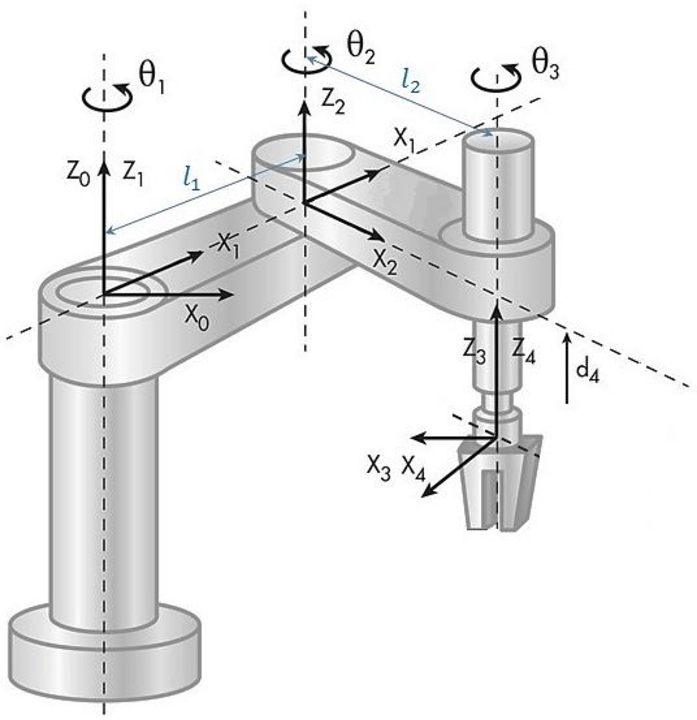
\includegraphics[width=0.5\textwidth]{SCARA-robot-of-4-gdl-Source-Our-elaboration.png}
% \caption{SCARA type manipulator. }
% \end{figure}

% What is the workspace volume for this robot?. (Draw a picture of it as well)
% \part[5] Write the DH parameters and forward kinematics for this robot 
% \part[10] Compute the inverse kinematics to get the robot to pick up an object at x=1.2, y=0.8, z=0.5

% \end{parts}
% \newpage

% You are tasked with surveying a remote agricultural area in Cote d'Ivoire which produces cocoa beans for top chocolate makers (yay chocolate!). Because of the costs of operation in this region of the world, you have been tasked with getting a robot to move from a base-station to survey a small patch of cocoa trees and estimate crop yeilds. 

% \noaddpoints
% \begin{parts}
% \part[5] What is the state space of the problem? What are the critical pieces of information that you feel is relevant to solving the problem? Are there any assumptions you are making in being able to access this information? Write this as a list, ie: State = ['something1', 'something2', ect.], assumptions = ['none', 'heroic assumption about amazing sensor', ect.]

% \part[10] Write your cost function? Does it have units? (If yes, what are they?) What are you penalizing/rewarding? Write this in the form of: Cost = <function>

% \part[10] What is a good heuristic function that can estimate your cost to accomplish this objective? (Note that this should be in the same units as your cost function.) What are the drawbacks and simplifications this function is making?

% \part[15] 
% What would your search algorithm look like? Illustrate the logic your system would follow to make a crop yeild estimate. (Draw a diagram of a few trees, where would your robot go first, how does your cost and heuristic fit together?) How much would you trust this information in making decisions about moving labor and resources here?


% \end{parts}

% \fillwithdottedlines{8em}

\end{questions}
\end{document}